    %---------------------------------------------------------------
        %% MLP
        %-----------------------------------------
        %% linkes Bild
\begin{tikzpicture}[>=stealth', node distance=\layersep cm, shorten >=1pt]
        \def\layersep{1.8}            % vertikal distance between the layers
        \def\neuronsep{1.8}         % Horizontal distance between neurons
        \def\dlsize{2}            % distance between node and layer lable
        \def\inout{\layersep*.65}   % Size of in- and output-arrow
        \def\siz{.8}                % neuronsize
        \def\y{5}                   % Start of the most upper layer
        \def\ni{3}                  % Amount of input neurons
        \def\nh{4}                  % Amount of hidden neurons
        \def\no{2}                  % Amount of output neurons
        \tikzstyle{neuron}=[circle,draw=black,minimum size=\siz cm,inner sep=2pt]
        \tikzstyle{annot} = [text width=6em, text centered]
        \tikzset{fontscale/.style = {font={\fontsize{#1pt}{#1pt}\selectfont}}}

        \newcommand{\neurono}[2][]{
            \node[neuron,circle split,inner sep=2pt] (#1) at (#2)
                    {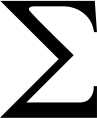
\includegraphics[width=0.225cm]{Bilder/Sigma.png} \nodepart{lower} 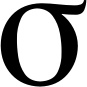
\includegraphics[width=0.225cm]{Bilder/sigma.png}};
        }
        % Draw the left input layer nodes
            \foreach \name / \xn in {1,...,\ni}{
            % This is the same as writing \foreach \name / \y in {1/1,2/2,3/3,4/4}
                \node[neuron,fontscale=15] (Il-\name) at (\xn*\neuronsep-\neuronsep,\y) {$i_{\xn}$};
                \node[above of=Il-\name, node distance=\inout cm] (Inl-\name) {};
                \draw [->,arrows={-Stealth[length=7pt]},densely dotted] (Inl-\name) edge (Il-\name);
            }
        % Draw the hidden layer node
            \foreach \name / \xn in {1,...,\nh}{
                \node[neuron,fontscale=15] (Hl-\xn) at ({(\ni-1)*\neuronsep/2-\neuronsep/2*(\nh-1)+(\xn-1)*\neuronsep},\y-\layersep) {$h_{\xn}$};
                \node[node distance=\inout cm, below of=Hl-\xn] (Hnl) {};
        % Connect every node in the inner layer with the hidden layer
            \foreach \source in {1,...,\ni}
                \draw [->,arrows={-Stealth[length=7pt]}] (Il-\source) edge (Hl-\xn);
                }
        % Draw the output layer node
            \foreach \name / \xn in {1,...,\no}{
                \node[neuron,fontscale=15] (Ol-\xn) at ({(\ni-1)*\neuronsep/2-\neuronsep/2*(\no-1)+(\xn-1)*\neuronsep},\y-2*\layersep) {$\Omega_{\xn}$};
                \node[node distance=\inout cm, below of=Ol-\xn] (Onl) {};
                \draw [->,arrows={-Stealth[length=7pt]},densely dotted] (Ol-\xn) edge (Onl);
        % Connect every node in the hidden layer with the output layer
            \foreach \source in {1,...,\nh}
                \draw [->,arrows={-Stealth[length=7pt]}] (Hl-\source) edge (Ol-\xn);
                }
        % Annotate the layers
            \ifthenelse{\ni>\nh}{
                \node[annot,right of=Il-\ni, node distance=\dlsize cm] (il) {\textbf{Eingabe- schicht}};
                \node[annot,below of=il] (hl) {\textbf{Verdeckte- schicht}};
            }{
                \node[annot,right of=Hl-\nh, node distance=\dlsize cm] (hl) {\textbf{Verdeckte- schicht}};
                \node[annot,above of=hl] (il) {\textbf{Eingabe- schicht}};
            }
                \node[annot,below of=hl] {\textbf{Ausgabe- schicht}};
        %-----------------------------------------
        %% rechtes Bild
            \tikzset{
                ident/.pic={
                \draw[semithick] (-\siz/4,-\siz/4) -- (\siz/4,\siz/4);
            }}
        % Draw the right input layer nodes
                \coordinate (tIr) at ($(il)-(Il-\ni)$);
                \coordinate (ttIr) at (tIr |- 0,0);
                \coordinate (Ir) at ($(il)+(ttIr)$);
            \foreach \name / \xn in {1,...,\ni}{
        % This is the same as writing \foreach \name / \y in {1/1,2/2,3/3,4/4}
                \node[neuron] (Ir-\name) at ($(Ir)+(\xn*\neuronsep-\neuronsep,0)$) {};
                \node[above of=Ir-\name, node distance=\inout cm] (Inr-\name) {};
                \pic at (Ir-\name) {ident};
                \draw [->,arrows={-Stealth[length=7pt]},densely dotted] (Inr-\name) edge (Ir-\name);
            }
        % Draw the right hidden layer node
            \foreach \name / \xn in {1,...,\nh}{
                \neurono[Hr-\xn]{$(Ir)+({(\ni-1)*\neuronsep/2-\neuronsep/2*(\nh-1)+(\xn-1)*\neuronsep},-\layersep)$}
                \node[node distance=\inout cm, below of=Hr-\xn] (Hnr) {};
        % Connect every node in the input layer with the hidden layer
            \foreach \source in {1,...,\ni}
                \draw [->,arrows={-Stealth[length=7pt]}] (Ir-\source) edge  (Hr-\xn);
            }            

                \node[fill=white,inner sep=1pt,fontscale=10] at ($(Hr-1)+({(\nh-1)*\neuronsep/2},\layersep*.5)$) {$\dots\,w_{i,h}\,\dots$};
        % Draw the right output layer node
            \foreach \name / \xn in {1,...,\no}{
                \neurono[Or-\xn]{$(Ir)+({(\ni-1)*\neuronsep/2-\neuronsep/2*(\no-1)+(\xn-1)*\neuronsep},-2*\layersep)$}
                \node[node distance=\inout cm, below of=Or-\xn] (Onr) {};
                \draw [->,arrows={-Stealth[length=7pt]},densely dotted] (Or-\xn) edge (Onr);
        % Connect every node in the hidden layer with the output layer
            \foreach \source in {1,...,\nh}
                \draw [->,arrows={-Stealth[length=7pt]}] (Hr-\source) edge  (Or-\xn);
            }
                \node[fill=white,inner sep=1pt,fontscale=10] at ($(Or-1)+({(\no-1)*\neuronsep/2},\layersep*.5)$) {$\dots\,w_{h,\Omega}\,\dots$};
\end{tikzpicture}